% https://phys.libretexts.org/Bookshelves/Modern_Physics/Book%3A_Spiral_Modern_Physics_(D'Alessandris)/4%3A_The_Photon/4.2%3A_Compton_Scattering
%https://courses.physics.ucsd.edu/2017/Spring/physics4e/compton.pdf
\documentclass{article}
\usepackage[utf8]{inputenc}
\usepackage{blindtext}
\usepackage{graphicx}
\usepackage{amsmath}
\usepackage{csvsimple}
\usepackage{pdfpages}
\usepackage{hyperref}
\usepackage{gensymb}

\begin{document}
\begin{center}
\textbf{\Huge{University of South Bohemia}}\\
\vspace{50px}
\textbf{\Large{Faculty of Science}} \\
\vspace{30px}
\includegraphics[width=120px]{~/school/logo.png} \\
\vspace{30px}
\textbf{\large{Praktika IV}}
\vspace{20px}
\\
\vspace{20px}
\large{Comptnův rozptyl} \\
\vspace{60px}
\end{center}
\begin{flushleft}
Datum: 18.10.2023 \\
Jmeno: Martin Skok \\
Obor: Fyzika \\
Hodnoceni:
\end{flushleft}
\newpage
\section{Úkoly}
\section{}
\section{Teorie}
Comptův rozptyl nastává, když dopadající foton má mnohem větší energii než elektron v atomu.
Když se pak tento foton srazí s elektronem jádře, může ho z jádra vyrazit a z elektronu se stane volný elektron.\\
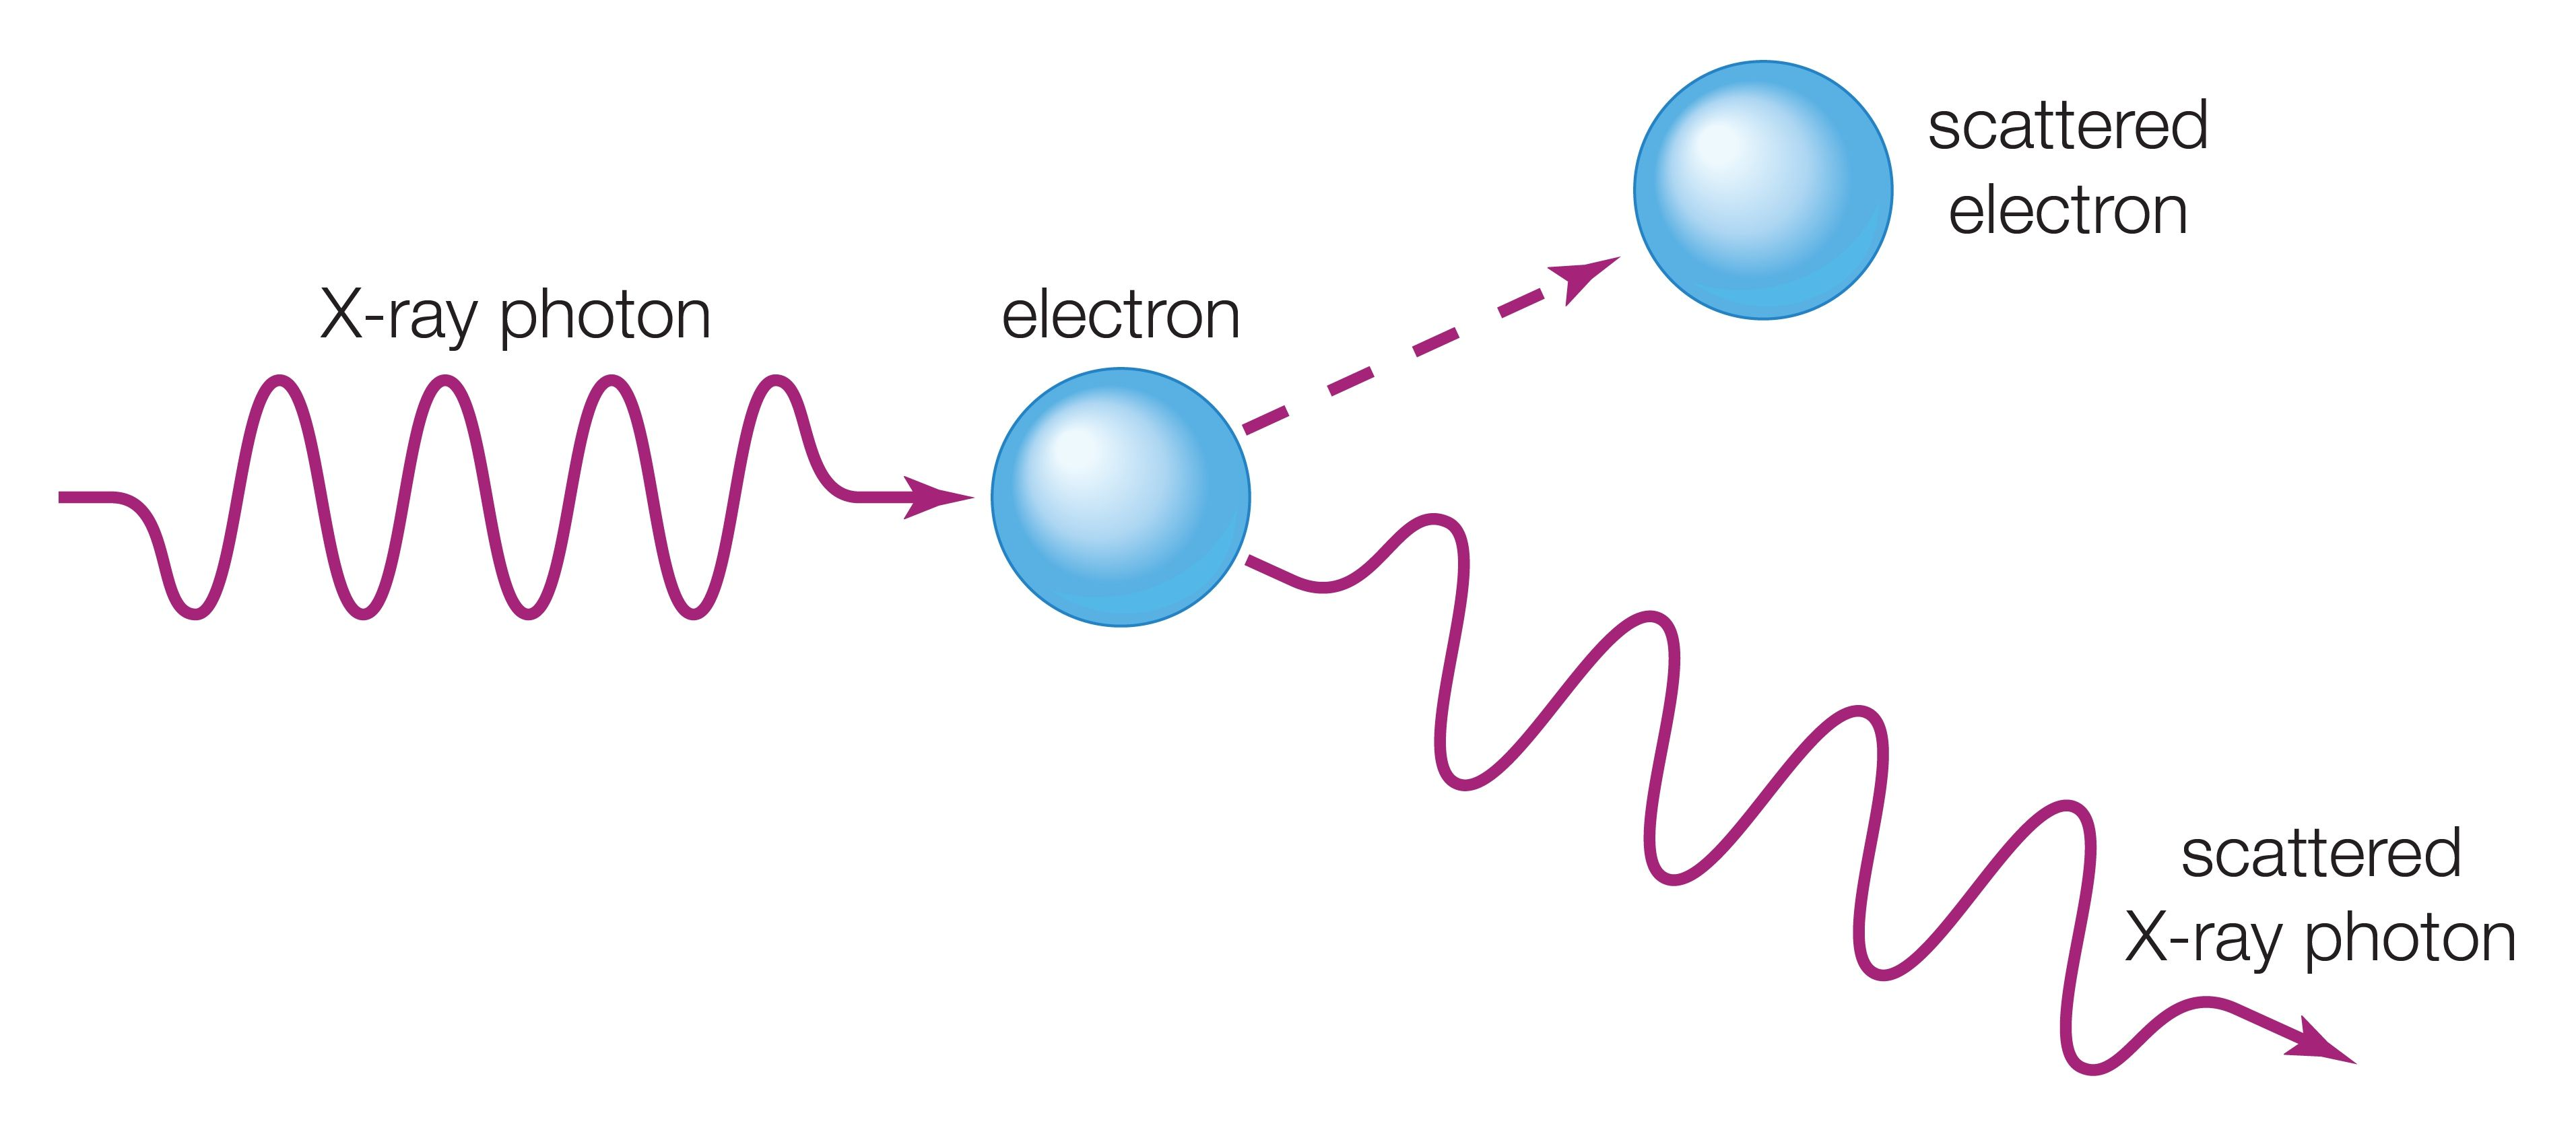
\includegraphics[scale=0.08]{comp.jpg}\\
Protože je mnohem jednoduší detekovat foton než elektron, parametry elektronu vyvodíme z vlastnotí rozptýleného fotonu.
$$p_{1} = p_{2} + p_{e}$$
Na vztah pro comptův rozptyl můžeme přijít ze zákona zachování energie, kde $p_{1}$ je hybnost fotonu před srážkou, $p_{2}$ je hybnost fotonu po srážce a $p_{e}$ je hybnost elektronu.\\
Nesmíme zapomenout, že hybnosti jsou vektory. Dále v textu už notaci vektorů nepoužívám.
$$(\vec{p}_{1} - \vec{p}_{2})^{2} = \vec{p}_{1}^{2} \vec{p}_{2}^{2} -2\vec{p}_{1}\vec{p}_{2}$$
$$(\vec{p}_{1} - \vec{p}_{2})^{2} = \vec{p}_{1}^{2} \vec{p}_{2}^{2} -2p_{1}p_{2}cos(\theta)$$
Potom bude úhel $\theta$ úhel rozptylu fotonem před srážkou a po srážce.\\
Pokud elektron bude před srážkou v klidu, bude mít energii $E_{0} = mc^{2}$, po srážce bude
mít energii $\sqrt{E_{0} + p^{2}_{e}c^{2}}$.
$$p_{1}c + E_{0} = p_{2}c + \sqrt{E_{0}^{2} + p_{e}^{2}c^{2}}$$
$$\vdots$$
\begin{equation}
  \lambda_{1} - \lambda_{2} = \frac{h}{mc} (1-cos\theta)
\end{equation}
$\lambda_{1}$ je vlnová délka nalétavajícího fotonu a $\lambda_{2}$ fotonu po srážce.

\end{document}
